\section{概览}\label{sec:Overview}
	YCSB(Yahoo! Cloud Serving Benchmark)是用来测试cloud serving/NoSQL/Key-Value Store的测试工具,代码开源,详细介绍见论文Benchmarking Cloud Serving Systems with YCSB。由于云服务的流行,传统数据库不能满足可利用性、可扩展性等要求,因此功能简化、一致性简化的NoSQL数据库逐渐流行。然而NoSQL数据库种类繁多,针对不同目的数据库各有权衡(读写性能、延迟和持久性、同步喝异步等等),用户和开发人员需要针对不同的应用场景选择合适的数据库。YCSB的目标是提供一个公平的平台,为这些数据库提供一个统一的测试方案,从而更公平地在不同的方面衡量不同的数据库性能,从而提供有价值的参考。

\section{YCSB应用模型}\label{sec:YCSB-Model}

	YCSB使用java编写,因为很多NoSQL系统拥有Java接口,其他没有Java接口的NoSQL系统可以通过比如HTTP/REST、JNI(Java Native Interface)等方式与java进行连接。由于KVF框架由c语言编写,所以在对KVF进行测试的时候需要用到JNI技术来实现KVF于YCSB的连接。

	YCSB模型图如下所示:

\begin{center}
	\includegraphics[width=13.9cm]{img/figure10.pdf}
\end{center}

	可以看出YCSB系统可以分为四个部分,分别是YCSB客户端,云数据库,任务集和命令行参数。

	\subsection{YCSB客户端}
		YCSB客户端是整个系统的核心,它包括任务集执行器,客户端线程,统计数据,和数据库客户端。

		YCSB客户端是一个用来产生数据和操作的Java程序,数据用来被加载到数据库中,操作包括读写更新删除等等,这些操作构成了任务集。基本的运行流程是任务集执行器驱动多个客户端线程,每一个线程执行一系列的操作,这些操作被标记为数据库接口层的调用,包括加载数据库(加载阶段)和执行任务集(交易阶段)。这些线程可以自行调节它们所产生的不同请求的比例,因此我们通过直接编写workload的方式来控制它。这些线程还会测量延迟和这些操作实现的吞吐量,并将这个测量数据报告到统计数据模块中,在每一次实验的结束,统计数据模块负责整合测量数据病报告前95\%的延迟和99\%的延迟。

		客户端将用一系列的属性(属性名/值对)来定义它的操作。通常情况下,我们将这些属性分为两组:
		\begin{itemize}
			\item \textbf{任务集属性}:
		用来定义任务集的一系列属性,独立于一个给定的数据库或者实验运行。比如指定对数据库读写操作的混合比例,指定分布方式,和记录的数量、大小和域的数目等等。
			\item \textbf{运行时属性}:
		是针对于一个给定的实验的属性集合,比如指定哪一种数据库(比如Cassandra、HBase等),指定初始化接口层的属性(比如数据库服务的主机名),指定客户端线程的数量等等。

		\end{itemize}
		
		因此任务集属性文件可以是静态的,并被应用于不同的不同数据库的测试实验中,运行时属性也一样可以存储在属性文件中,但是真对不通的实验、数据库和目标吞吐量这些属性的值可能会大有不同。

	\subsection{Workload}
		workload指的是测试数据库系统时需要完成的任务集,在YCSB系统中自带六个workload,分别针对不用的应用场景

		Workload A: 更新操作权重很高的任务集

				这个任务集是由50\%的读操作和50\%的写操作混合而成,一个典型的应用例子是会话存储记录最近的行为。

		Workload B: 几乎全是读操作的任务集

				这个任务集由95\%的读操作和5\%的写操作混合而成,应用场景为照片打标签,添加标签是更新操作,但是绝大部分的操作是读取tag

		Workload C: 全部是读写的任务集

				这个任务集100\%是读,应用例子是用户简介的缓存,用户的简介实际上是在其他地方创建的。

		Workload D: 读最近的任务集

				在这个任务集中,新的记录被插入,最新插入的记录是最经常被读取的。一个典型的应用例子:用户更新,其他用户想要看到的是最新修改的内容。

		Workload E: 短的排列

				在这个任务集中,一小排记录被查询,而不是一个单独的记录,应用例子:一段对话,每一次扫描

		Workload F: 读-修改-写

				在这个任务集中,客户端将读一个记录,修改它,然后写回。应用例子:用户数据库,用户读取自己的记录然后

	\subsection{JNI}
		The Java Native Interface (JNI) 是一个Java软件开发工具的一个原声编程接口,通过它可以使得Java代码使用其他语言编写的代码和代码库,比如C和C++。 Invocation 接口是JNI的一部分,可以用来讲Java虚拟机(JVM)嵌入到原生应用中国年,从而允许其他语言的原生应用可以调用Java代码。

		在benchmarkd实现的过程中,需要以下工具:

		Java编译器:javac执行命令需要SDK

		Java虚拟机:java执行命令需要SDK

		原生方法C文件产生器:javah命令需要SDK

		定义了JNI的库文件和原生头文件:C头文件jni.h、jvm.lib、jvm.dll或者jvm.so都需要SDK

		可以产生共享库的C和C++编译器:在linux系统下cc编译器是最常见的

		在Java 2 SDK中,Java虚拟机和Java运行时支持位于共享库中的libjvm.so

		连接YCSB和KVF需要如下六步:

		编写Java代码。我们需要首先编写Java类来完成三个任务:声明将要调用的原生方法,加载包含原生代码的共享库,调用原生方法。

		编译Java代码。在使用之前我们必须成功将Java类编译成为二进制代码。

		创建C头文件。头文件中声明我们想调用的原生函数,这个头文件将用来和C函数实现一起创建共享库。

		写C代码,这一步需要实现C源代码,该文件必须包含在第三步创建的头文件。

		创建共享库文件。我们将从第4步获得的C源代码文件创建共享库文件。

		运行Java程序。

		为了对比KVF底层接于nvmkv后的功能和性能,我分别编写了Makefile来对KVF和nvmkv进行基本的测试,Makefile的实际上是指定了编译规则以及依赖关系,在每一个编译指令的最开始会指定生成对象的名称,然后指定生成该文件所依赖的文件名,在第二行指定编译工具以及编译细节,在编写Makefile时需要将最后编译的文件在最前面指出,因此整个Makefile的罗列顺序和实际的编译顺序是相反的。如下代码是列出了测试nvmkv时Makefile中关键的步骤,我将按照实际的编译顺序进行介绍。

		\begin{Verbatim}[frame = single]
	com/yahoo/ycsb/db/JNvmkv.class : com/yahoo/ycsb/db/JNvmkv.java
    javac com/yahoo/ycsb/db/JNvmkv.java

		\end{Verbatim}
		首先编译JNvmvk对象,这个类对nvmkv的底层函数进行了封装,供YCSB client调用。


		\begin{Verbatim}[frame = single]
	com/yahoo/ycsb/db/com_yahoo_ycsb_db_JNvmkv.h \ 
	com/yahoo/ycsb/db/JNvmkv.class
    javah -classpath . -d ./com/yahoo/ycsb/db/ \ 
        com.yahoo.ycsb.db.JNvmkv

		\end{Verbatim}
		这一步生成负荷JNI格式的头文件,其中每一个函数名都以com\_yahoo\_ycsb\_db\_开头,在编写Jnvmkv.c文件时,函数名要和这里的保持一致。



		\begin{Verbatim}[frame = single]
com.yahoo.ycsb.db.com_yahoo_ycsb_db_JNvmkv.o : \ 
	com/yahoo/ycsb/db/JNvmkv.c \ 
	com/yahoo/ycsb/db/nvmkv-test.h
    g++ -c $< -o com/yahoo/ycsb/db/com_yahoo_ycsb_db_JNvmkv.o\ 
        $(LDFLAGS) -I/usr/lib/jvm/java/include/ -I/usr/lib/jvm/\ 
        java/include/linux/ -fPIC
		
		\end{Verbatim}
		这一步生成目标文件,用于最终生成共享函数库文件。


		\begin{Verbatim}[frame = single]
com.yahoo.ycsb.db.libcom_yahoo_ycsb_db_JNvmkv.so : \ 
	com/yahoo/ycsb/db/com_yahoo_ycsb_db_JNvmkv.h : \
	com.yahoo.ycsb.db.com_yahoo_ycsb_db_JNvmkv.o
    gcc -I/usr/lib/jvm/java/include/\
        -I/usr/lib/jvm/java/include/linux/ \
        -L$(PATH_TO_ANANAS_LIB) $(LDLIBS) $(LDFLAGS)\
        -fPIC -o com/yahoo/ycsb/db/libcom_yahoo_ycsb_db_JNvmkv.so\ 
        -shared -Wl,-soname,com/yahoo/ycsb/db/\
        com_yahoo_ycsb_db_JNvmkv.so com/yahoo/ycsb/db/\
        com_yahoo_ycsb_db_JNvmkv.o
    javah -classpath . -d ./com/yahoo/ycsb/db/ \ 
        com.yahoo.ycsb.db.JNvmkv

		\end{Verbatim}
		这一步最终生成YCSB Client在运行时会调用的共享函数库文件。

		\begin{Verbatim}[frame = single]
run :
        java -Djava.library.path=$(PATH_TO_YCSB)YCSB/nvmkv/src/\
        main/java/com/yahoo/ycsb/db/\
        com.yahoo.ycsb.db.JNvmkv
		
		\end{Verbatim}
		在最终使用YCSB测试之前,我做了一个单独的基本功能测试,在运行时需要指定库文件路径,一遍调用上一步编译出来的共享函数库文件。

	\subsection{实现方式}
		YCSB是一套完整的测试系统,我们需要将KVF当作YCSB的一个数据库模块添加到YCSB中。YCSB的数据库接口层隐藏了所在做测试的NoSQL数据库的细节,这就允许客户端产生像“读记录”“更新记录”这样简单的操作,而不用理解你所指定数据库的特定接口。因此,YCSB很容易来测评一个新加入的数据库系统。一旦你创建了数据库接口层,YCSB框架的其他地方不需要做任何改变就可以顺利运行。

		YCSB的数据库接口层是一个简单的抽象类,为你的数据库提供了读、插入、更新、删除和扫描操作。为KVF实现一个数据库接口层只需要实现这具体的函数体,一旦这个接口层可以顺利编译,我们就可以在命令行(或者属性文件中)指定为KVF实现的类名。因此我们并不需要因为添加或者更改了数据库接口耳重新编译YCSB客户端。

		根据下列步骤即可完成KVF模块的创建

		\begin{Verbatim}[frame = none]
    第一步:继承 com.yahoo.ycsb.DB		
		\end{Verbatim}

		该类是所有数据库接口层实现的基类,它是一个抽象类,所以我们需要实现一个继承于com.yahoo.ycsb.DB的类,在这类我们把这个类声明为AnanasClient,这个类需要拥有一个无参数的构造函数,因为在AnanasClient的实例将会在YCSB内部通过无参数的构造函数生成。

		YCSB客户端框架会为AnanasClient的每一个线程都创建一个实例,但是我们需要测试多线程的功能,所以会有多个工作者线程都产生任务集,每一个线程都会创建一个AnanasClient实例。

		\begin{Verbatim}[frame = none]
    第二步:实现init()如果有必要的话
		\end{Verbatim}
		
		通过下面的方法我们可以初始化我们的DB对象:

		public void init() throws DBException

		该方法在每个AnanasClient实例中都会被调用一次,所以如果在测试的时候使用多线程的方式,每个AnanasClient实例都会被各调用一次。

		init()方法应该被用来连接数据库和其他相关初始化工作。需要指出的是,YCSB提供了一种可以在运行时使用属性文件配置数据库的方式。事实上,YCSB客户端会在启动的时候将在属性文件指定的所有参数文件都传递到数据库接口层。因此,我们可以为数据库接口层创建新的属性文件来,在参数文件中或者命令行中进行设置,然后在我们自己实现的AnanasClient中获得这个参数文件并设置相应的属性。

		这些属性将会在构造函数被调用后传递到实例中,因此我们需要在init()方法中获得这些属性而不是在构造函数中,我们可以调用下列方法,该方法已经被实现并从DB基类继承而来。


		\begin{Verbatim}[frame = none]
    第三步:实现数据库查询更新方法
		\end{Verbatim}

		下列方法是AnanasClient需要实现的:

		\begin{Verbatim}[frame = single]
  //Read a single record
  public int read(String table, String key, Set<String> fields, 
  HashMap<String,String> result);

  //Perform a range scan
  public int scan(String table, String startkey, int recordcount, 
  Set<String> fields, Vector<HashMap<String,String>> result);
	
  //Update a single record
  public int update(String table, String key, HashMap<String,
  String> values);

  //Insert a single record
  public int insert(String table, String key, HashMap<String,
  String> values);

  //Delete a single record
  public int delete(String table, String key);

		\end{Verbatim}
		在每一次调用的时候,这些方法都会使用一个表名称和记录的键。对于读和扫描方法,需要额外外的参数来提供一个数据结构存储返回的数据。对于插入和更行方法来说,需要传入映射了域名和值的哈西映射(HashMap)。

		数据库应该在运行测评之前创建号合适的表。我们在实现上述方法的时候认为适当的表已经存在,只需要从指定的表中读和写。

		在这里我将介绍KVF对应的YCSB Client的实现细节。
\begin{center}
	\includegraphics[width=13.9cm]{img/figure11.pdf}
\end{center}
		
		如上图所示,JAnanasClient是一个YCSB Client的实例,它继承了com.yahoo.ycsb.DB类,并实现了需要实现的函数,在实现的过程中使用JAnanas类进行具体的对数据库的操作,JAnanas类将KVF封装成为一个数据库,并通过JNI与JAnanas.c进行连接,从而调用KVF中实现的接口,达到访问数据库的目的。		

		\begin{Verbatim}[frame = none]
    第四步:编译数据库接口层
		\end{Verbatim}

		我们的代码可以独立于YCSB客户端和YCSB框架单独编译,因此当我们对自己的数据库接口层AnanasClient作修改之后只需编译自己的模块而不用重新编译YCSB客户端。


		\begin{Verbatim}[frame = none]
    第五步 测试数据库	
		\end{Verbatim}

		YCSB提供了简单的命令行客户端来测试接口层,它创建一个数据库实例,允许你世界操作数据库而不用启动一个任务集,例子如下:

\begin{Verbatim}[frame = single]

% java com.yahoo.ycsb.CommandLine -db com.yahoo.ycsb.db.MongoDbClient 
-p mongodb.url=mongodb://localhost:27017 -p mongodb.database=ycsb

YCSB Command Line client
Type “help” for command line help
Start with “-help” for usage info
Connected.
> insert brianfrankcooper first=brian last=cooper
Return code: 1
191 ms
> read brianfrankcooper
Return code: 0
last=cooper
_id=brianfrankcooper
first=brian
2 ms
> quit
\end{Verbatim}

		首先使用命令行工具以及相关的参数启动一个数据库,然后进行单独的插入、读、更新、删除等操作,这样即可自行验证功能的正确性。比如在上述实例中,首先插入一条记录,id为brianfrankcooper,第一个值为brian,第二个值为cooper,然后读取记录,读出的信息和插入的一样,验证成功。


		\begin{Verbatim}[frame = none]
	第六步:使用YCSB客户端测试
		\end{Verbatim}

		使用YCSB集成测试需要在YCSB项目的根目录下运行ycsb的python脚本,在命令行指定数据库和任务集以及线程等相关信息。

	\subsection{实现流程}

	1.在YCSB中新建一个文件kvf/,将KVF作为一个新的Database添加到YCSB框架中

	2.在YCSB/kvf/目录下新建pom.xml文件用于编译,文件内容和YCSB中其他database的相应文件一样,只需做与kvf相关的修改即可

	3.在YCSB/kvf/目录下仿照其他database的目录结构新建src/main/java/,在这个目录下创建Makefile用于简化编译过程

	4.在YCSB/kvf/src/main/java目录下新建com/yahoo/ycsb/db/目录结构,实现java的包结构方便进行编译

	5.在这个目录下新建文件AnanasClient.java,该类继承了com.yahoo.ycsb.DB类,在该类中重写了一些关键的方法来供YCSB的上层测试函数的调用

	6.创建JAnanas.java用于对kvf的包装

		因为kvf用c语言编写,YCSB为java编写,所以需要使用Java Native Interface来将其连接

	7.通过JAnanas.java编译出头文件com\_yahoo\_ycsb\_db\_JAnanas.h

	根据编译出的头文件编写com\_yahoo\_ycsb\_db\_JAnanas.c实现JAnanas.java中的native函数

	8.在YCSB/bin中的ycsb脚本文件第75行添加kvf

	9.在YCSB/pom.xml中添加kvf

	10.在distribution/pom.xml中添加kvf

	\subsection{测试计划}
	在图形界面客户端中进行测试
	对多线程进行测试:将线程数分别设置为1,2,4,8,16,21,64,128分别测试
。

	通过参数设置配置不同读、插入、更新、删除操作比例的测试文件进行测试:例如:不同读写比率(100\%插入、90\% 更新+ 10\%读、65\%读+25\% 插入+10\% 更新、90\% 读+10\% 插入、100\%读等)

	如下我可以自定义任务集,指定操作数、插入、更新、读取、删除的比例,以及分布方式:
\begin{Verbatim}[frame = single]
    workload=com.yahoo.ycsb.workloads.CoreWorkload
    readallfields=false
    readproportion=0.65
    updateproportion=0.25
    scanproportion=0
    insertproportion=0.1
    requestdistribution=uniform
\end{Verbatim}

	在这个任务集中首先会将1000个记录加载到数据库中,在实际测试的时候将有2000次操作,读取数据的比例是65\%,更新的比例为25\%,插入的比例为10\%,分布方式为全部随机分布,在命令行中指定线程数为16.

	通过YCSB的stat结构统计数据,我们可以得到如下的测试结果:

\begin{Verbatim}[frame = single]
[OVERALL], RunTime(ms), 516.0
[OVERALL], Throughput(ops/sec), 3875.968992248062
[CLEANUP], Operations, 1.0
[CLEANUP], AverageLatency(us), 5.0
[CLEANUP], MinLatency(us), 5.0
[CLEANUP], MaxLatency(us), 5.0
[CLEANUP], 95thPercentileLatency(us), 5.0
[CLEANUP], 99thPercentileLatency(us), 5.0
[INSERT], Operations, 216.0
[INSERT], AverageLatency(us), 554.5185185185185
[INSERT], MinLatency(us), 283.0
[INSERT], MaxLatency(us), 1852.0
[INSERT], 95thPercentileLatency(us), 961.0
[INSERT], 99thPercentileLatency(us), 1554.0
[INSERT], Return=0, 216
[READ], Operations, 1302.0
[READ], AverageLatency(us), 89.02150537634408
[READ], MinLatency(us), 34.0
[READ], MaxLatency(us), 701.0
[READ], 95thPercentileLatency(us), 206.0
[READ], 99thPercentileLatency(us), 288.0
[READ], Return=0, 1302
[UPDATE], Operations, 482.0
[UPDATE], AverageLatency(us), 143.00829875518673
[UPDATE], MinLatency(us), 69.0
[UPDATE], MaxLatency(us), 841.0
[UPDATE], 95thPercentileLatency(us), 236.0
[UPDATE], 99thPercentileLatency(us), 298.0
[UPDATE], Return=0, 482
\end{Verbatim}

	从结果中我们可以看到,吞吐量为3875.96op\/s,由于有16个线程所以会清除16次。

	插入操作有216次,平均延迟为554.51us,最大一次延迟为1852.0us,最小的一次延迟为283.0us,99\%的插入延迟在1554.0us以内,95\%的插入延迟在961.0us\%以内。

	读操作有1302次,平均延迟为89.02us,最大一次延迟为701.0us,最小的一次延迟为34.0us,99\%的读延迟在288.0us以内,95\%的读延迟在206.0us\%以内。


	更新操作有482次,平均延迟为143.00us,最大一次延迟为841.0us,最小的一次延迟为69.0us,99\%的读延迟在298.0us以内,95\%的读延迟在236.0us\%以内。

	为了更近直观地分析和对比数据,我将YCSB的测试结构进行可视化处理。

\begin{center}
	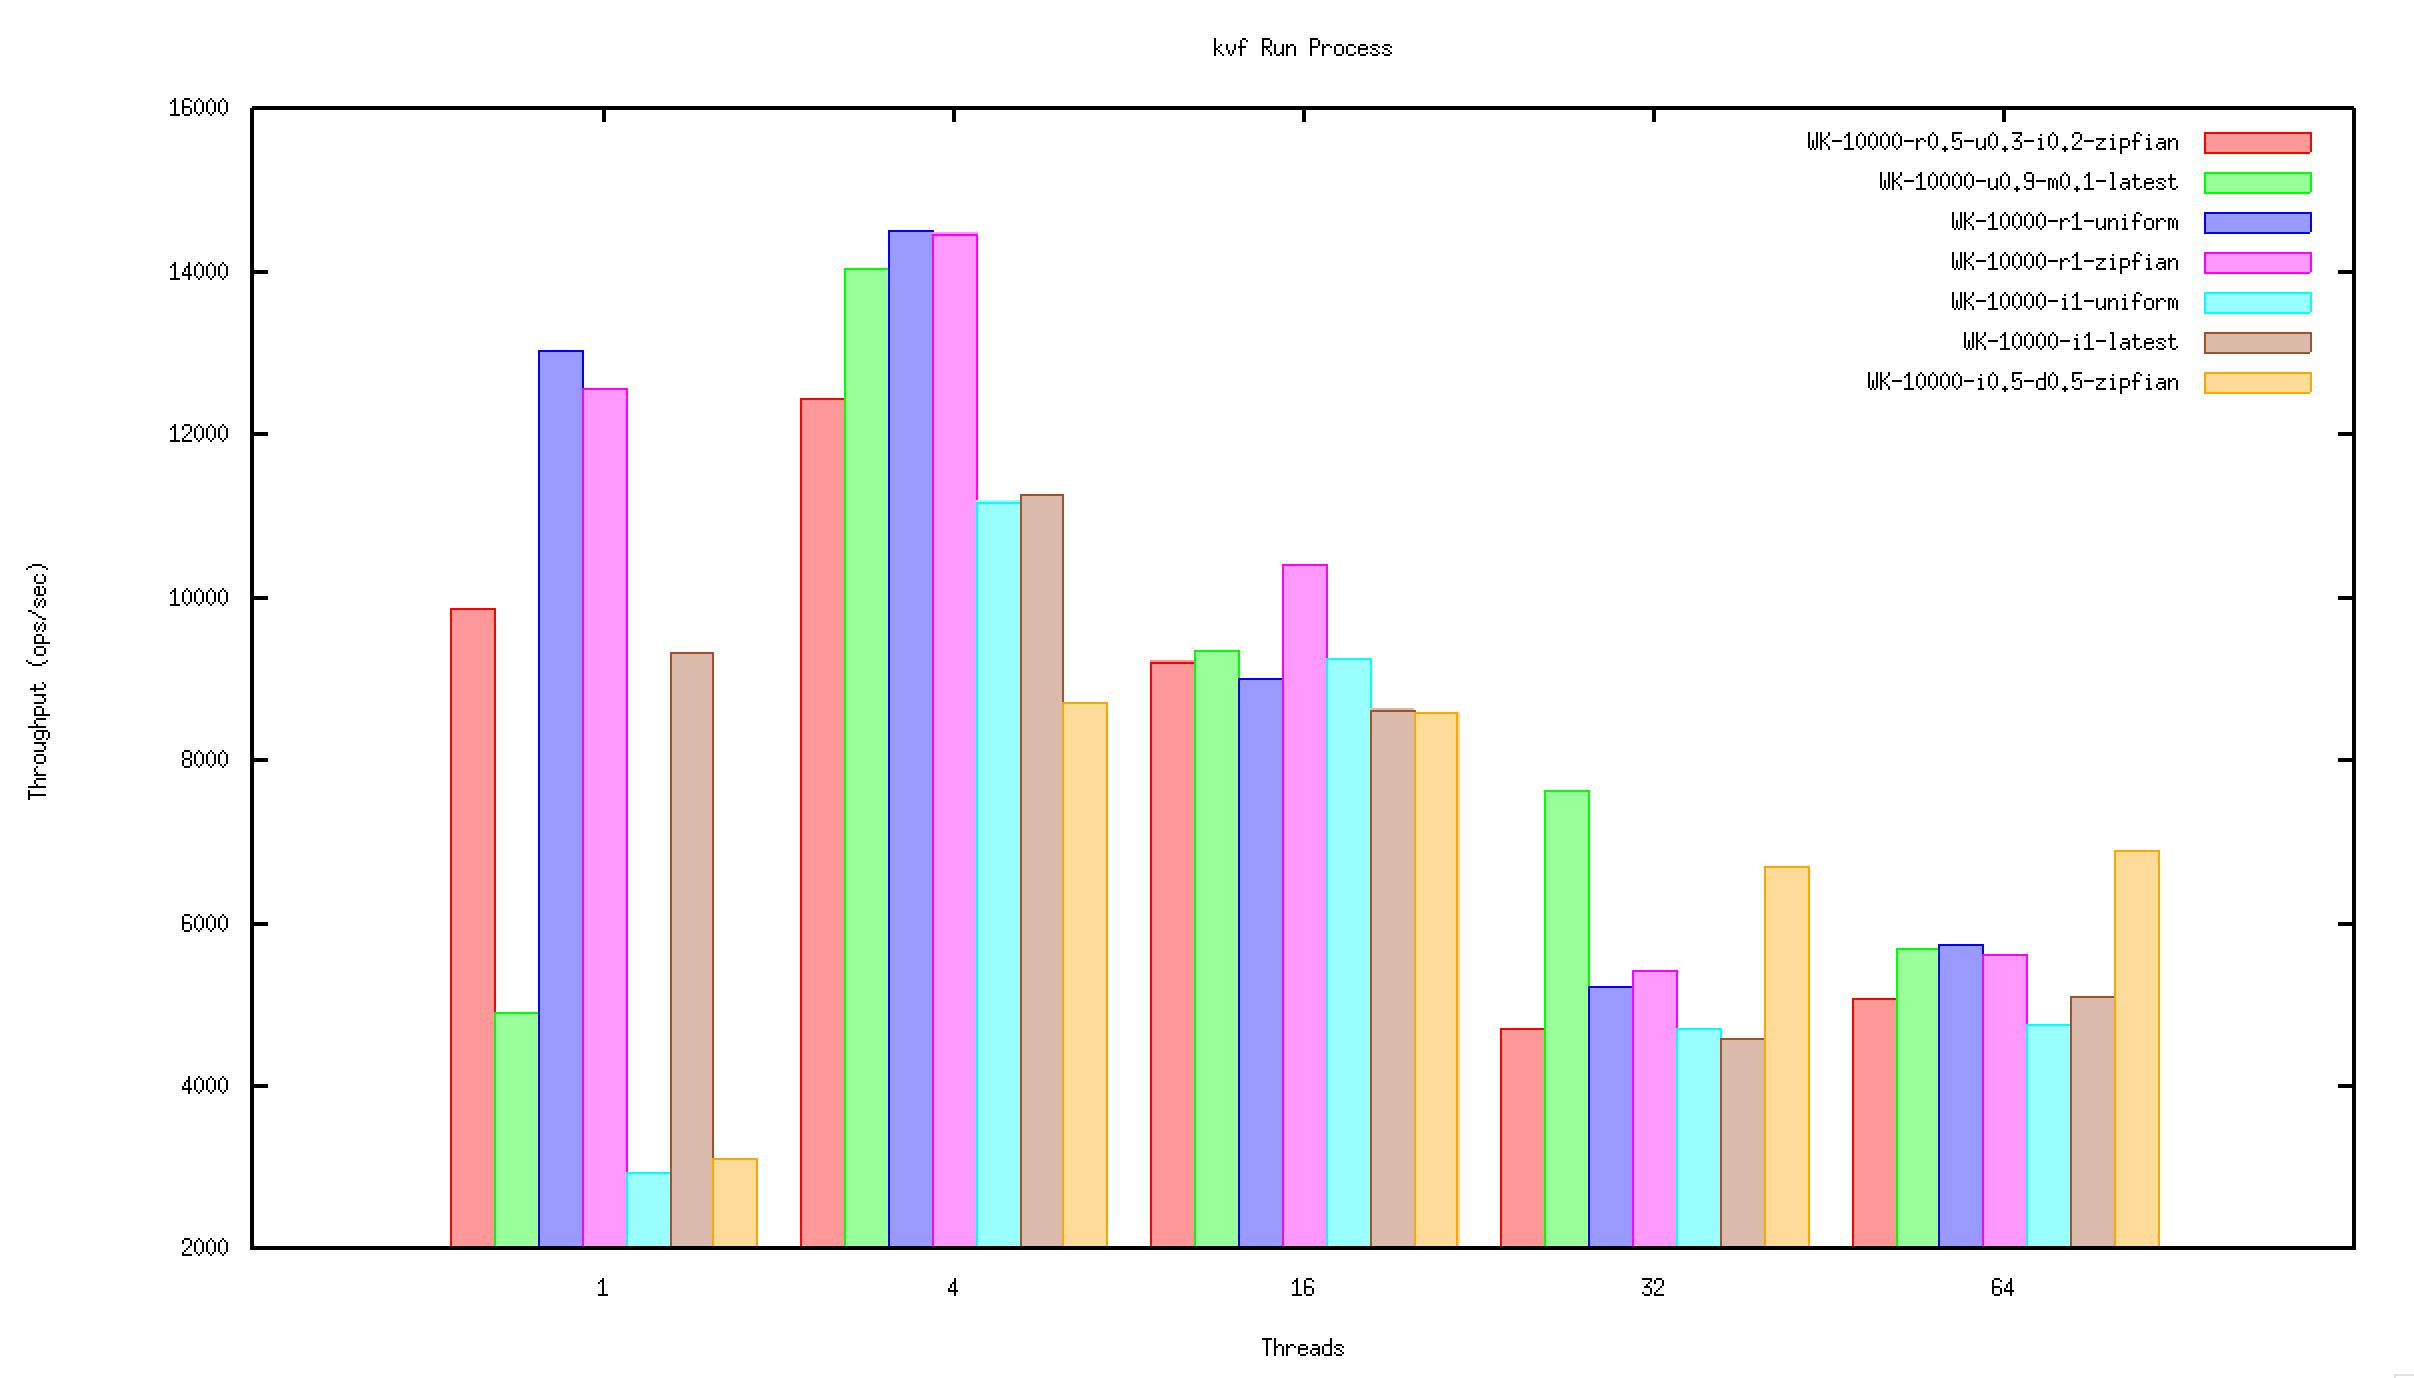
\includegraphics[width=13.9cm]{img/figure14.pdf}
\end{center}

	图中测试了六种不同的任务集分别在1、4、16、32、64线程中总体的吞吐量统计图。除了总体的数据,还可以短读显示插入、读、删除等每一种操作单独的统计数据。

\begin{center}
	\includegraphics[width=13.9cm]{img/figure15.pdf}
\end{center}

	该图是同样测试的延迟统计。可以看出当线程数增加时延迟会越来越大。



%     - public int read(String table, String key, Set<String> 
%     - public int update(String table, String key, HashMap<String,
% public int update(String table, String key, HashMap<String,
%     - public void init() throws DBException {} 
%     - public int insert(String table, String key, HashMap<String,
	
%  public int read(String table, String key, Set<String> fields, 

% public int insert(String table, String key, HashMap<String,
% public int delete(String table, String key);
%     - public int delete(String table, String key);
% public int scan(String table, String startkey, int recordcount,

% java com.yahoo.ycsb.CommandLine -db com.yahoo.ycsb.db.MongoDbClient 

% 		\includegraphics[width=15cm]{img/figure15.pdf}
% 	% 		\includegraphics[width=13.9cm]{img/figure13.pdf}、
% 		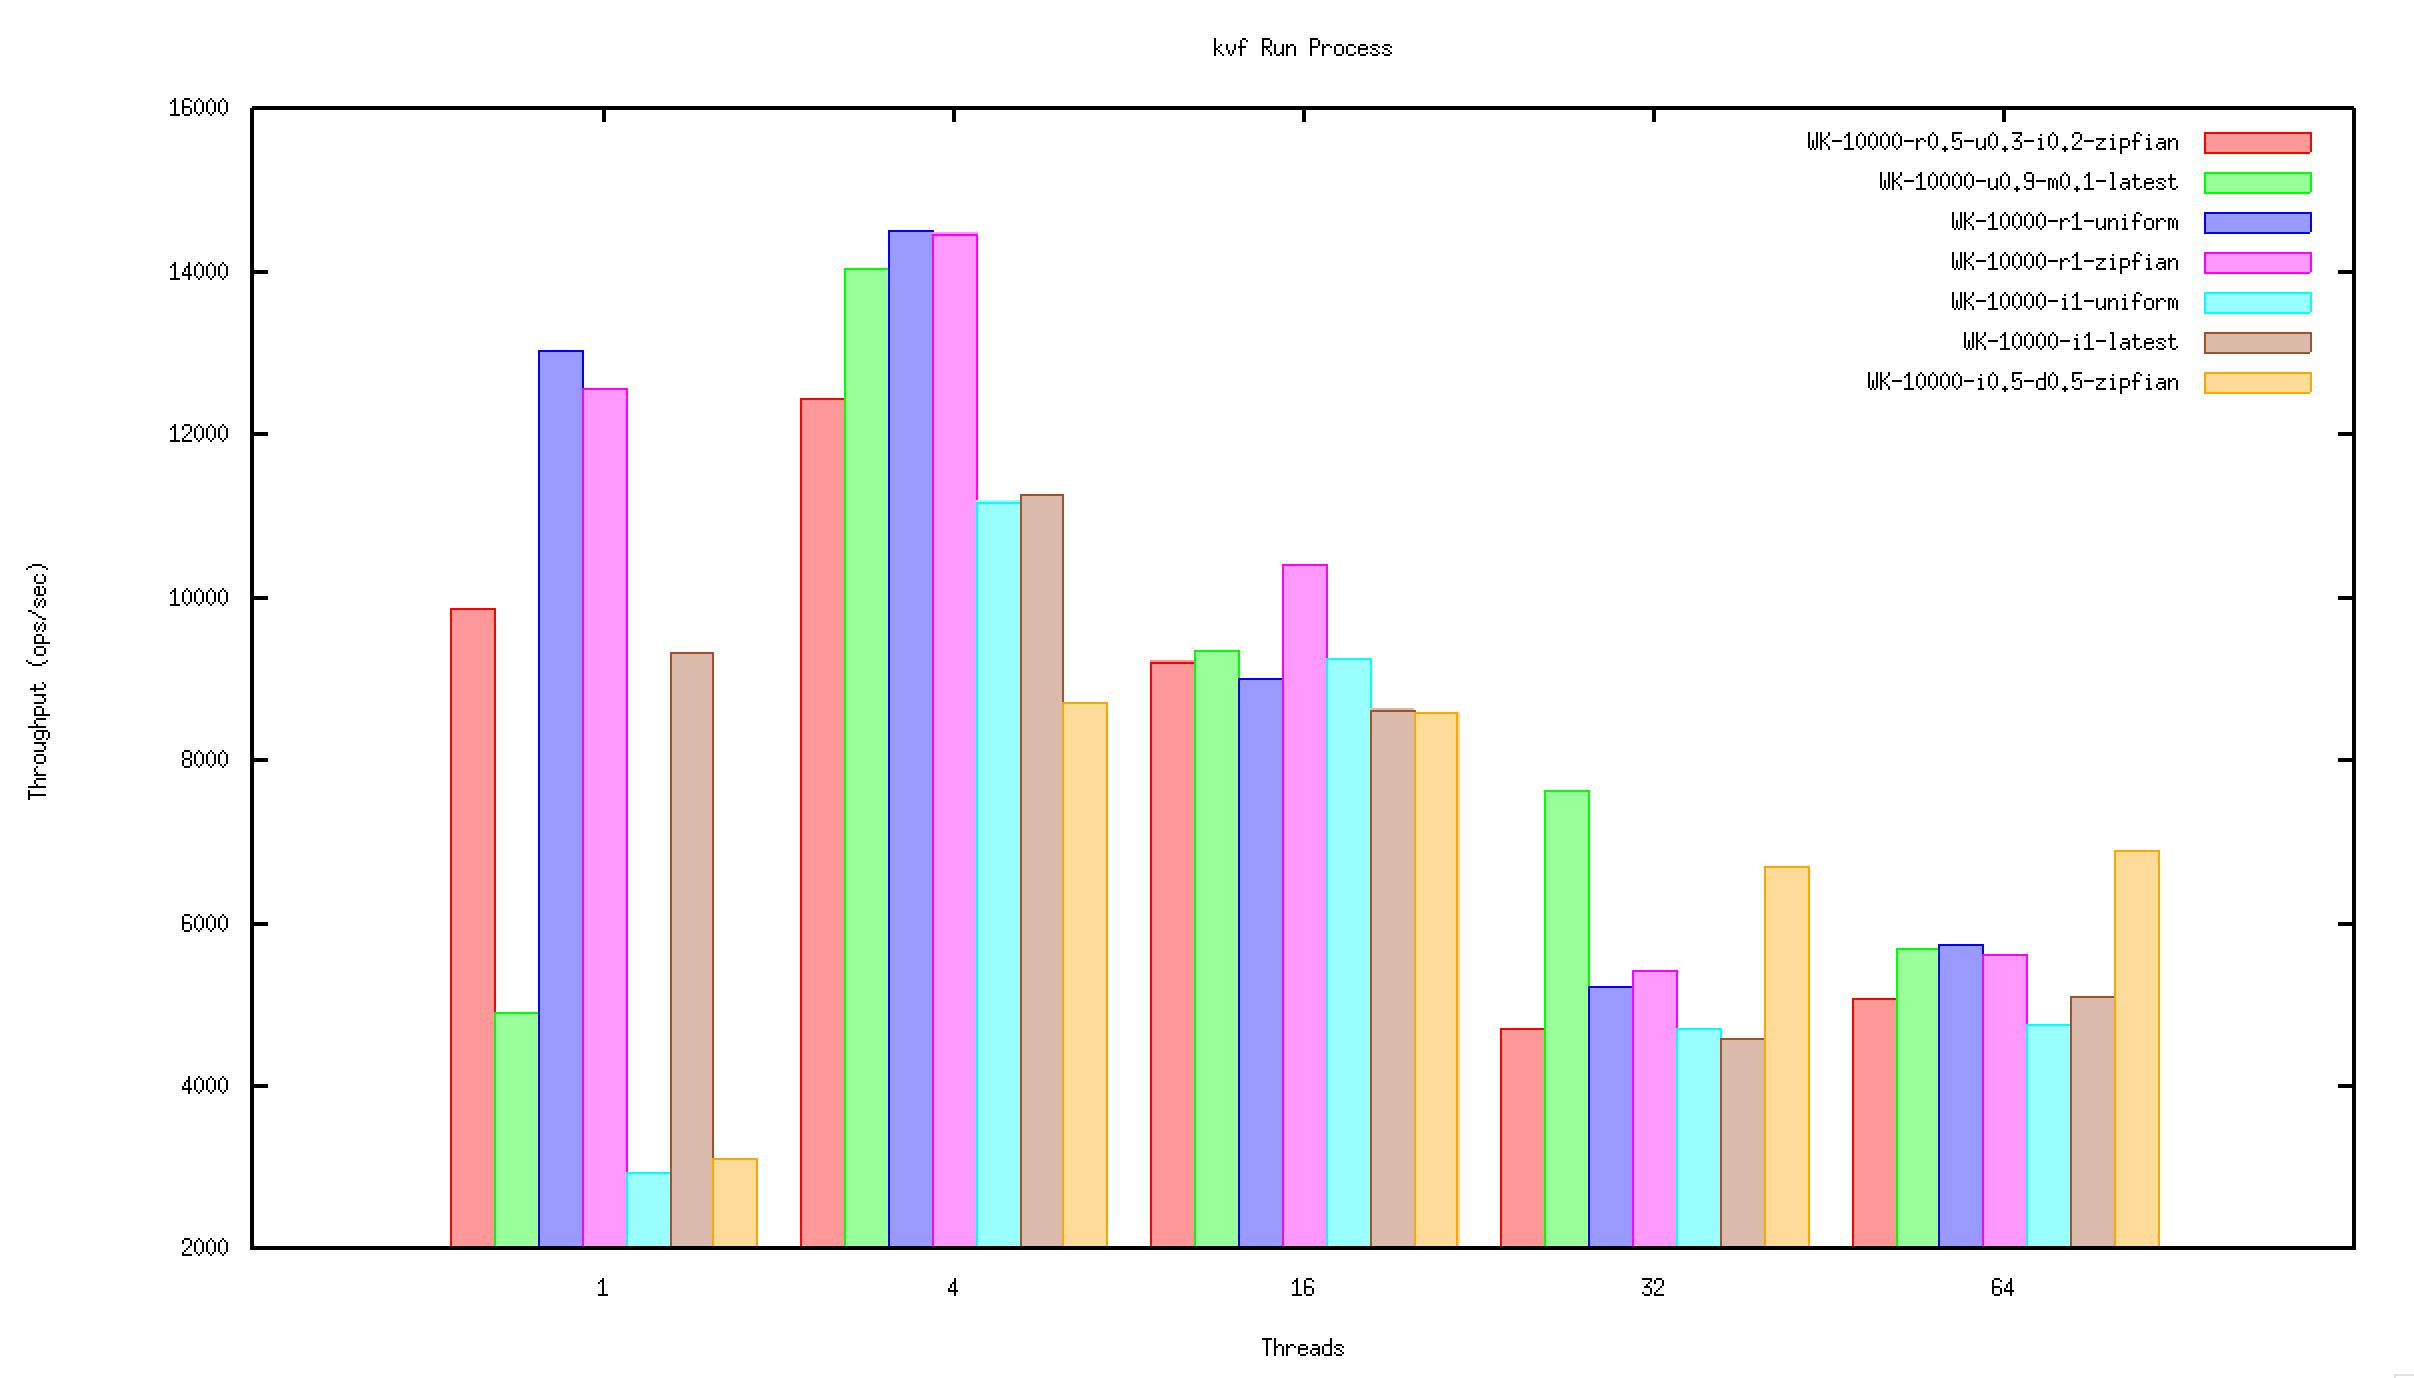
\includegraphics[width=15cm]{img/figure14.pdf}












%     [OVERALL], RunTime(ms), 309.0


	
%  	HashMap<String,String> result);

	

%     [UPDATE], AverageLatency(us), 1453.1361940298507


% 2 ms


	


% 	该方法对kvf进行初始化
%     String> values);
	
		


	


%     [UPDATE], 95thPercentileLatency(us), 2529.0
% 		\end{Verbatim}
% 191 ms
		
%     fields, HashMap<String,String> result);


%     operationcount=2000
	
% Type “help” for command line help

% Return code: 0




% //Insert a single record
% Return code: 1
		
%     [UPDATE], MaxLatency(us), 3625.0
%     [READ], Return=0, 1248

	
% //Update a single record
%     [INSERT], Operations, 216.0
%     [UPDATE], 99thPercentileLatency(us), 3119.0
	

%     [CLEANUP], 95thPercentileLatency(us), 1.0
%     [INSERT], AverageLatency(us), 2446.527777777778
% 	插入一个key/value对

% Connected.
% 	\end{center}



% 	删除一个key/value对





% 		\end{center}
% 		\end{Verbatim}
% 	\end{Verbatim}

%     [INSERT], Return=0, 216


% 	% 	\end{center}
%     [READ], MaxLatency(us), 7715.0
%     [OVERALL], Throughput(ops/sec), 6472.491909385113
%     [UPDATE], MinLatency(us), 208.0
%     readallfields=true
%     [INSERT], MaxLatency(us), 7903.0



% 	% \begin{center}



% 		\end{Verbatim}
%     requestdistribution=uniform
%     [INSERT], MinLatency(us), 643.0

  		
%     [READ], AverageLatency(us), 1267.5753205128206


% % vim:ts=4:sw=4


%     [UPDATE], Return=0, 536
		

	
% 	\begin{Verbatim}[frame = single]
		
		
	
%     [READ], 95thPercentileLatency(us), 2401.0
%     recordcount=1000
% 	\end{center}



% > insert brianfrankcooper first=brian last=cooper







% 	String> values);








% 	\end{Verbatim}
% \chapter{KVF测试系统YCSB}
%     updateproportion=0.25
	

% 		\end{Verbatim}



% //Delete a single record



% 		\end{Verbatim}
		
% 	Set<String> fields, Vector<HashMap<String,String>> result);

%     [READ], 99thPercentileLatency(us), 6383.0
%     readproportion=0.65

% 		\end{Verbatim}

%     workload=com.yahoo.ycsb.workloads.CoreWorkload
% 		\end{Verbatim}
% YCSB Command Line client

%     [CLEANUP], AverageLatency(us), 1.375


			
% 		\end{Verbatim}
% 		\begin{Verbatim}[frame = single]
% > quit
% 	String> values);
% 	\begin{center}
% 	更新一个记录

%     [CLEANUP], Operations, 16.0

%     [READ], MinLatency(us), 96.0
%   	String> values);
% 		\begin{Verbatim}[frame = single]
%     [CLEANUP], MinLatency(us), 0.0
  		
		
% 		\begin{Verbatim}[frame = single]

% 	\begin{Verbatim}[frame = none]
% 	\begin{Verbatim}[frame = none]
	
% 	\end{Verbatim}
		


% last=cooper
% % \pkuthssffaq % 中文测试文字。
% 	在给定的table中查找某个key对应的value



		
% first=brian
% 		\begin{Verbatim}[frame = single]

	
%     [READ], Operations, 1248.0
%     [INSERT], 95thPercentileLatency(us), 3661.0
% 		\begin{Verbatim}[frame = single]



% Start with “-help” for usage info
% 	\begin{Verbatim}[frame = none]
% 	\begin{center}
%     [INSERT], 99thPercentileLatency(us), 4455.0

% -p mongodb.url=mongodb://localhost:27017 -p mongodb.database=ycsb
	

%     [CLEANUP], MaxLatency(us), 9.0
% 		\end{Verbatim}
% //Perform a range scan
% 	\begin{Verbatim}[frame = single]


	

%     insertproportion=0.1
%     [UPDATE], Operations, 536.0
% \_id=brianfrankcooper

	
% 	\begin{Verbatim}[frame = none]
% 	\begin{Verbatim}[frame = single]
%     [CLEANUP], 99thPercentileLatency(us), 9.0
% 		\begin{center}


		
	
		
% > read brianfrankcooper



% 		\end{Verbatim}




% 		\begin{Verbatim}[frame = single]




%  //Read a single record